\section{Implementation}
\begin{figure}[t!]
    \centering{}
	\subfloat[Architecture] { 
    	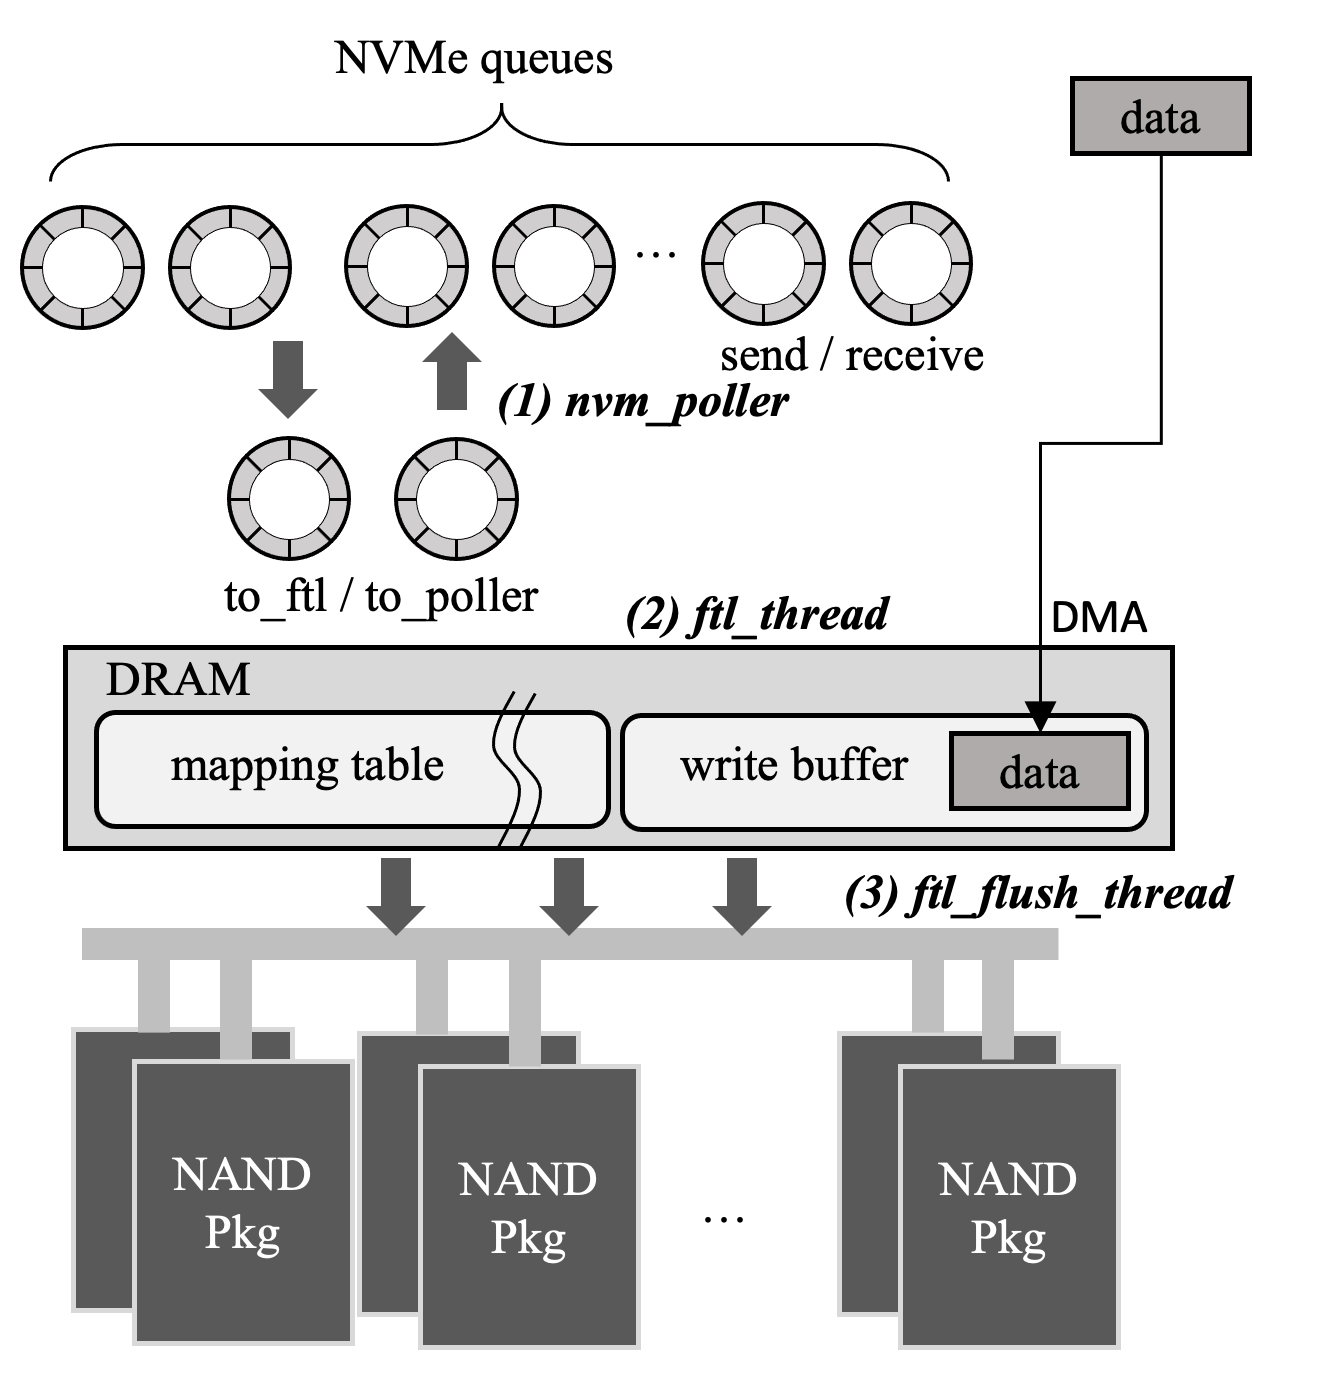
\includegraphics[width=0.3\textwidth]{figure/dawid_ssd_archi_new.eps}
	} \\
	\subfloat[Data structures for FTL]{ 
    	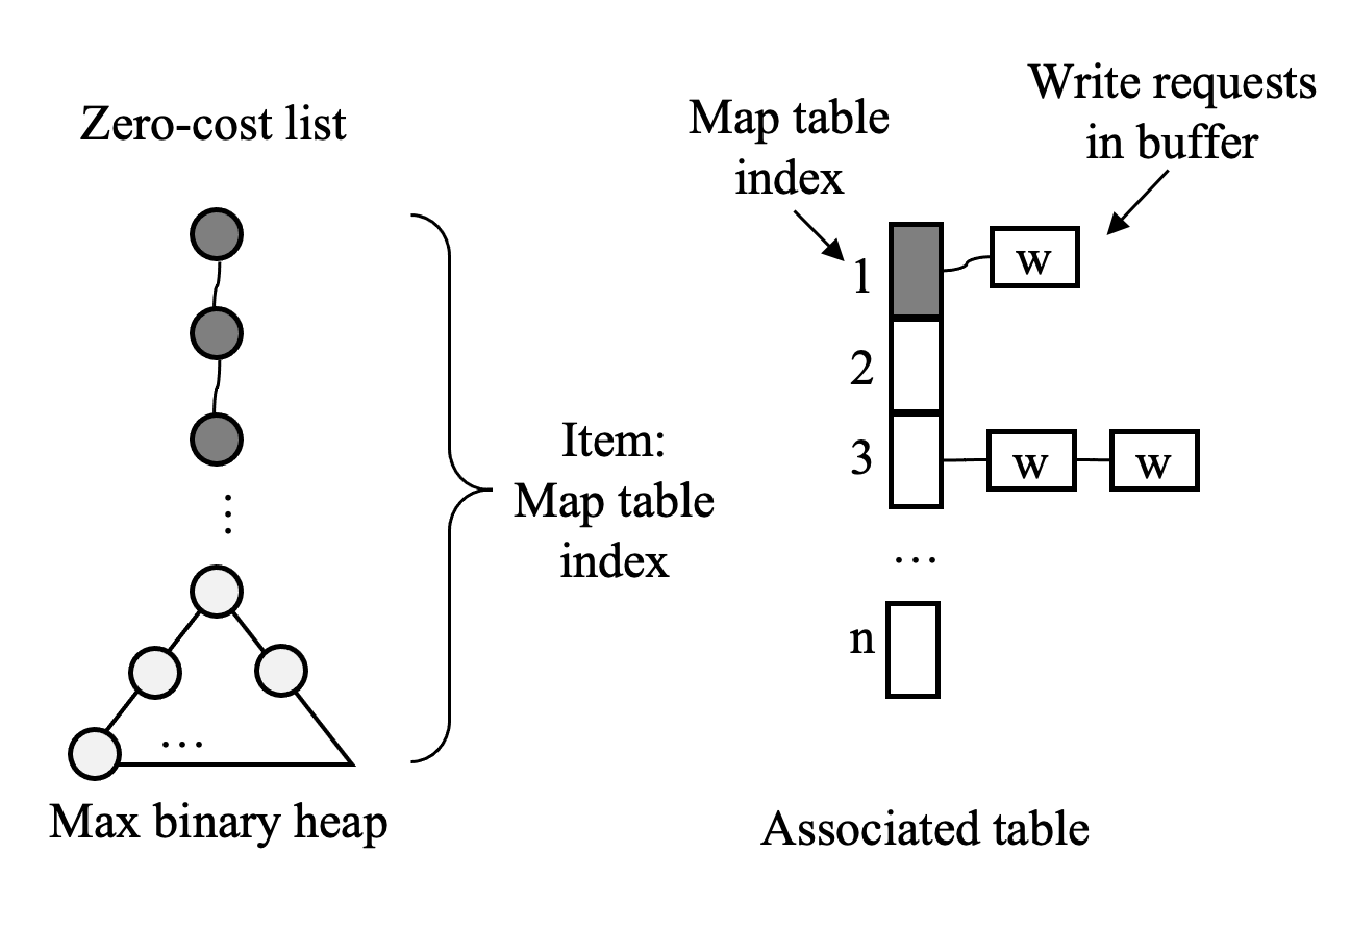
\includegraphics[width=0.3\textwidth]{figure/dawid_ds.eps}
	}
    %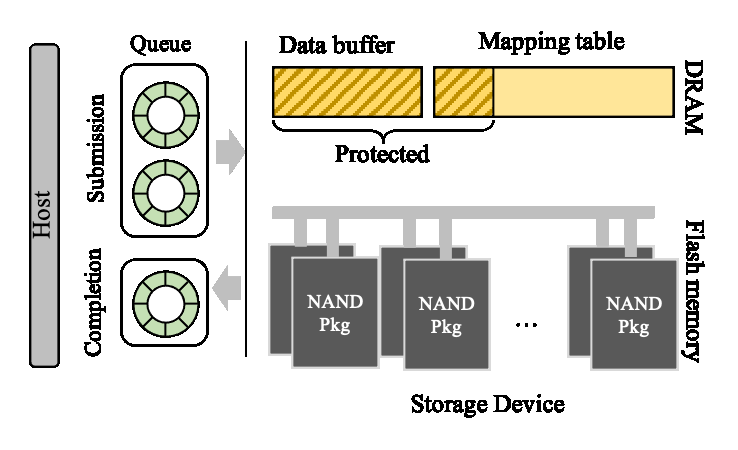
\includegraphics[width=0.4\textwidth]{figure/dawid_ssd_archi.eps}
    \caption{\textbf{\ours{}-SSD} Internals.}
    \label{fig_dawid_archi}
\end{figure}


\begin{figure*}[!t]
    \centering{}
	\subfloat[Random] { 
	    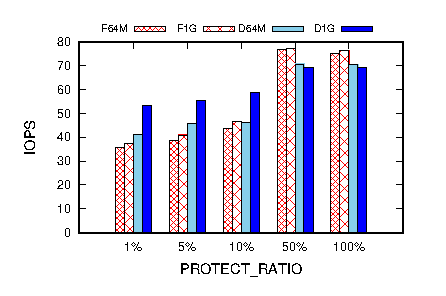
\includegraphics[width=0.3\textwidth]{expr/micro_rslt_220525/perf/perf_RAND.eps}
	} 
	\subfloat[JESD] { 
	    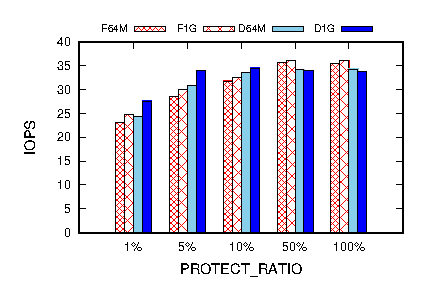
\includegraphics[width=0.3\textwidth]{expr/micro_rslt_220525/perf/perf_JESD.eps}
	}
	\subfloat[TPC-C] {
	    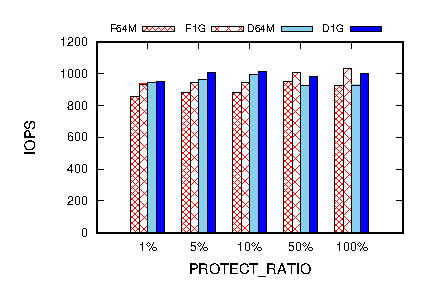
\includegraphics[width=0.3\textwidth]{expr/macro_rslt_220525/perf/perf_OLTP.eps}
	}
    \caption{\textbf{IOPS}:\textit{F and H denotes FIFO and HEXA.}}
    \label{fig_perf_iops}
\end{figure*} 


\begin{figure*}[!t]
    \centering{}
	\subfloat[Random] { 
	    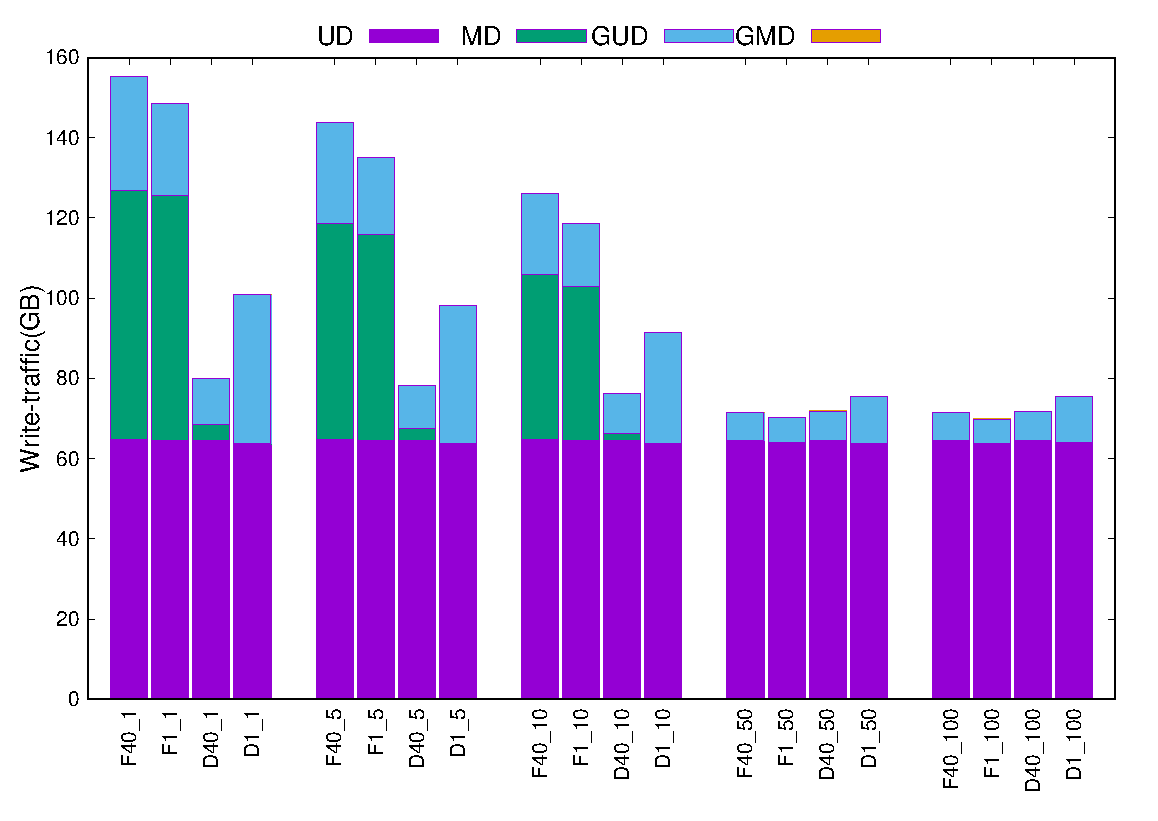
\includegraphics[width=0.28\textwidth]{expr/micro_rslt_220525/wt/RAND.eps}
	} 
	\subfloat[JESD] { 
	    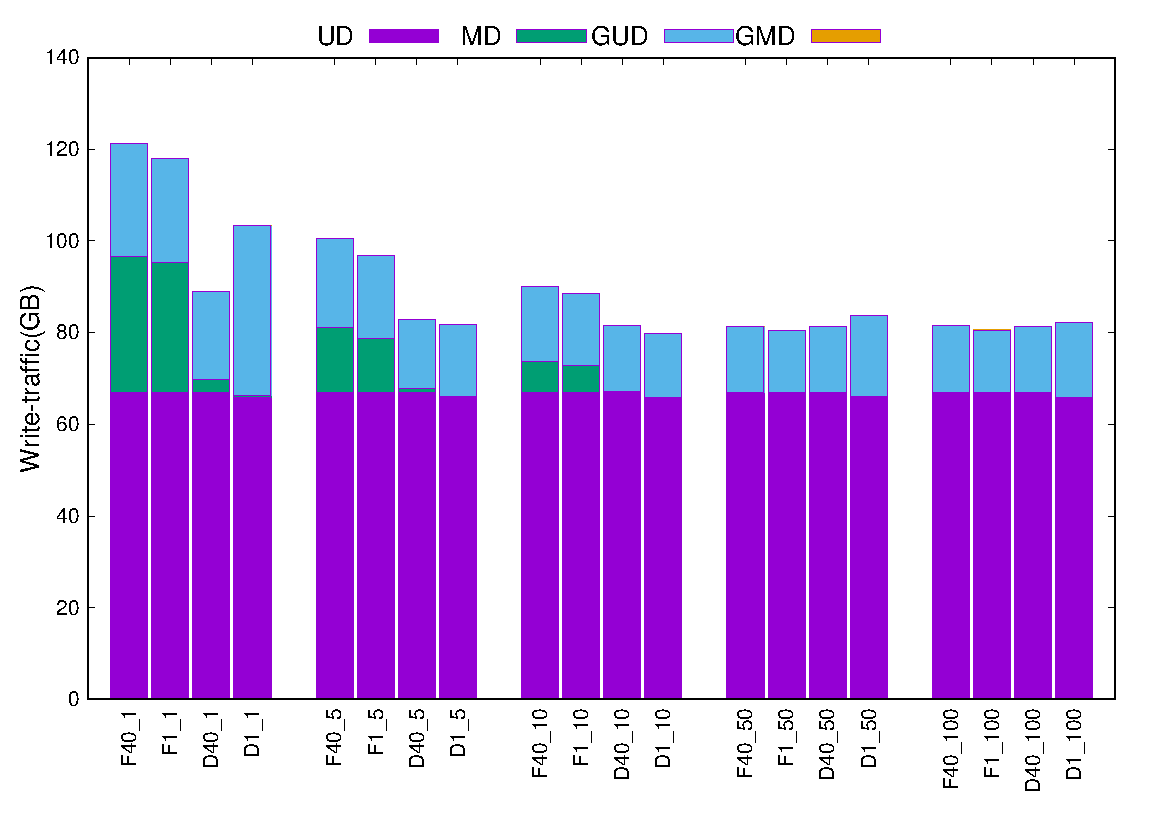
\includegraphics[width=0.28\textwidth]{expr/micro_rslt_220525/wt/JESD.eps}
	}
	\subfloat[TPC-C] { 
	    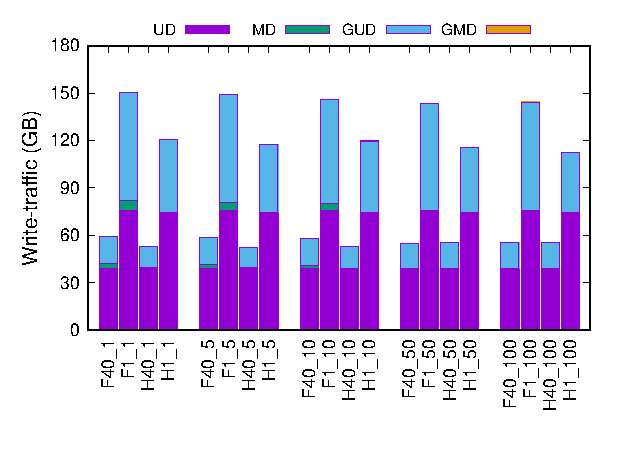
\includegraphics[width=0.28\textwidth]{expr/macro_rslt_220525/wt/OLTP.eps}
	}
	\caption{\textbf{Write Traffic.} \textit{UD - User Data, MD - Mapping Data,
				GUD - GC Write for User Data, GMD - GC Write for Mapping Data.}}}
    \label{fig_perf_wt}
\end{figure*} 



We implement \ours{} in \texttt{FEMU}, an open-source SSD development
framework~\cite{li2018case}. Fig.~\ref{fig_dawid_archi} shows the overall
architecture of \ours{}-SSD and its internal data structures. As the original
version of \texttt{FEMU} directly writes data to flash memories without write
buffering, we extend it to use a small-sized write buffer, which aggregates and  
batches user writes into the underlying flash memory.  

\ours{}-SSD maintains three different threads that are executing concrrently
within SSDs.  The \texttt{nvm\_poller} takes a charge of transferring requests
between NVMe queues and FTL-internal queues. The FTL-internal queue consists of
a pair of sub-queues, each of which is named \texttt{to\_ftl} and
\texttt{to\_poller}). This separation is intended to enable a non-blocking
access to queues by allowing only a single writer for each queue.  Second, the
\texttt{ftl\_thread} essentially handles the ingress requests from the internal
queues. For write, it transfers data from the host memory to the SSD-internal
write buffer with DMA and updates the associated entry in a translation page to
point to the write buffer. Then, it notifies the completion of request to the
\texttt{nvm\_poller} by enqueueing the acknowledgement into the
\texttt{to\_poller} queue.  Because \ours{} protects the entire space of write
buffer with capacitance, data persistency is guaranteed for all acknowledged
writes.  For read, the \texttt{ftl\_thread} retrieves the requested data by
consulting the mapping table and transfers it to the host. 

The \texttt{ftl\_flush\_thread} plays a role of writing data from a DRAM-buffer
into a flash memory.  With the \texttt{FIFO} policy, the user writes are issued
to NAND flash memory in the order they arrive into the buffer. However, \ours{}
flushes buffered writes in the order such that it least increases the dirty memory
footprint of the mapping table.  To realize this design, \ours{} maintains two
data structures, as depicted in Fig.~\ref{fig_dawid_archi}(b). First, \textit{a
zero-cost list} that holds the indexes to tranlsation pages that is already
in a dirty state, and second, \textit{a max binary heap} that
maintains the indexes to translation pages sorted by the number of buffered
user write requests associated with that page.  

%When there is sufficient bandwidth at underlying NAND flash subsystem for writes, 
When a half of the write buffer becomes occupied, flushing is invoked. \ours{}-SSD
first flushes user data whose translation pages in the zero-cost list, and then
persists user data as their translation pages are ordered by the max binary
heap. By doing so, each user write minimizes the number of eventual
translation page write, and each translation page write maximizes the number of
persisted mapping entries. These data structures are updated by the \texttt{ftl\_thread} 
when a write request arrives at SSD. 
To exploit the SSD internal parallelism, we send data to flash memory in
batches by the number of NAND flash chips that can be written simultaneously.

Once the write operations of NAND flash memory complete,
\texttt{ftl\_flush\_thread} updates the mapping table entries to point to the
physical address of the data in a flash memory.  At this moment, if the number
of dirty mapping table pages goes beyond the protectable number of pages,
\texttt{ftl\_flush\_thread} persists the mapping table page to flash memory.
This is also conducted in batches by the number of NAND flash chips that can be
written in parallel.


\section{Evaluation}
%We assume 1\% of the mapping table is protected via capacitors in a 64GB SSD. 
%The 64GB SSD is using DRAM and assumes that 1\% of the mapping table is
%protected. 
We perform the experiments on a machine with a 20-core Intel Xeon(R) Silver
4114 CPU running at 2.2GHz and 84GB memory. We run FEMU (QEMU-based SSD
emulator) configured to use 10 cores, 4GB DRAM for main memory, and 16GB DRAM
for SSD emulation. The SSD maintains a mapping table entirely in DRAM partially
protected with capacitance. The NAND flash chips include 8 channels and 8 flash
LUNs per channel. The page size is 8KB and the per-block pages are 256. The
read and write latency is set to 60us and 700us,
respectively~\cite{cheong2018flash}. We use the greedy algorithm for
GC(Garbage-Collection), which selects the least utilized block as a victim for
cleaning. The Ext4 file system is mounted on the emulated SSD.  
%Other configuration uses default settings of FEMU 

We measure the average IOPS and the write traffic varying the protected ratio
of a mapping table from 1\% to 100\%. We study two different sizes of write
buffer, 64MB and 1GB, to investigate the effectiveness of \ours{} with respect
to a queue depth. The performance evaluation is conducted using three workloads.
The fio benchmark~\cite{fio-bench} generates the 4KB of random writes and the
skewed read-write mixed workload that follows JESD219 using 4 threads. A
total of 64GB of data was written to the 4GB area. For the real workload, we use 
TPC-C~\cite{council1990tpc} on MySQL, an online transactional processing benchmark, 
which is executed using a sysbench benchmark suite~\cite{sysbench}.
The TPC-C preconditions an SSD with data writes for 300 seconds and generates  
write quries for 180 seconds using 10 threads.
For the performance comparison, we also implemented an FIFO-SSD, which uses 
a FIFO(First-In-First-Out) scheduling policy for processing write requests within SSDs. 

Fig.\ref{fig_perf_iops} show the IOPS of FIFO-SSD and \ours{}-SSD with different size of write buffers, and Fig.~\ref{fig_perf_wt} shows the write traffic breakdown for the scenario.
When the protected ratio is less than 10\%, \ours{} has improved the performance by up to XX\% compared to the existing FIFO version.
Compared with full protection SSD, when the protected ratio is 1\%, FIFO performance degradation occurs more than XX\%-XX\%, whereas in \ours{}, performance degradation is XX\% - XX\%. This performance enhancement is achieved by significantly reducing the cost of flushing overflew dirty pages to the SSD through the in-buffer re-ordering.
\iffalse
protected ratio 가 10\% 이하일 때 DAWID 이 기존 FIFO 방식 버전보다 최대 XX\%
성능을 향상시켰다.  Full protected 경우와 비교하면 protected ratio 가 1\%로
줄어들 때 FIFO는 성능저하가 XX\%-XX\% 이상 발생하는 반면, DAWID은 성능저하가
XX\% - XX\% 에 머물렀다.  이러한 성능향상 효과는 mapping table 의 영속성을 위해
dirty page 를 SSD에 flush 하는 오버헤드를 in-buffer re-ordering 을 통해 상당히
많이 줄였기 때문이다. 
Fig.~\ref{fio_perf_wt}에서 보는바와 같이 DAWID은 protected ratio 가 작을 때에도
mapping table flush 오버헤드를 거의 없애 FIFO 대비 쓰기량을 최대 XX\%까지 절감하였다. 
\fi

\iffalse
한가지 예상치 못한 결과는 protected ratio 가 50\% 이상일 때 DAWID이 FIFO보다
IOPS가 살짝 낮다는 것이다. In-depth analysis 를 수행한 결과 reordering 이 host
에서 발생시키는 본연의 write pattern 을 distort 하게 되는데 이로 인해 lifetime
이 다른 page 들이 동일 블록에 저장되는 가능성을 높이기 때문이다. 결과적으로
이는 GC에서 copy 해야 하는 valid page 의 숫자를 증가시켜 GC의 write traffic 을
늘린다.  워크로드가 synthetic random 인 상황에서도 파일시스템을 거쳐서 들어오기
때문에 temporal locality 를 가짐. 이에 re-ordering 을 통한 host write pattern
의 왜곡이 GC의 성능 저하를 일으키게 됨. 본 논문에서 targeting 하는 상황은
protected ratio 가 낮은 경우이지만 기법의 적용성(?)을 향상시키기 위해 상기 문제를 
완화시킬 수 있는 기법에 대해 향후 연구해보고자 합. 
\fi

One counter-intuitive result is that \ours{} has slightly lower IOPS than FIFO when protected ratio is above 50\%. Our careful analysis reveals that the reordering of \ours{} distorts the original write pattern generated by the host, which increases the possibility that pages with different lifetimes are stored in the same block. As a result, this increases the number of valid pages that need to be copied from the GC, thereby increasing the write traffic of the GC. Even when the workload is synthetic random, the host writes have temporal locality because they are transferred through a file system. Therefore, distortion of host write pattern through re-ordering causes degradation of GC performance. Note that the target environment of this paper is a case where the protected ratio is low, but in order to improve the generality of \ours{}, we will study the technique that can alleviate the above problem in the future.


%\begin{figure*}[t]
%    \centering{}
%	\subfloat[OLTP] { 
%	    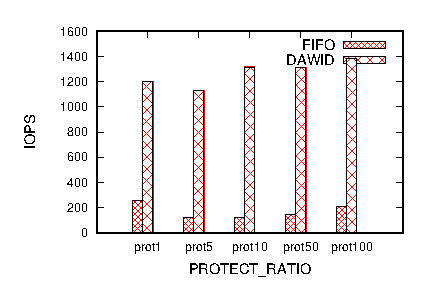
\includegraphics[width=0.3\textwidth]{expr/macro_220517/perf/OLTP/perf_OLTP.eps}
%	} 
%	\subfloat[Write Traffic] { 
%	    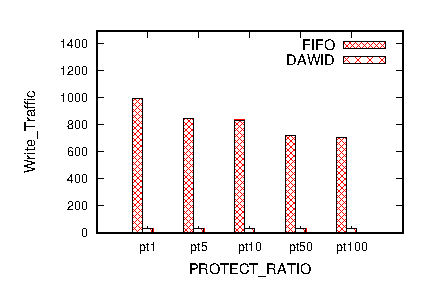
\includegraphics[width=0.3\textwidth]{expr/macro_220517/wt/OLTP/perf_OLTP.eps}
%	} 
%    \caption{\textbf{OLTP}}
%\end{figure*} 



%\begin{figure*}[t]
%    \centering{}
%	\subfloat[Sequential] { 
%	    %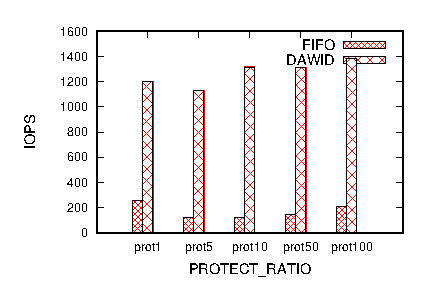
\includegraphics[width=0.3\textwidth]{expr/macro_220517/perf/OLTP/perf_OLTP.eps}
%	    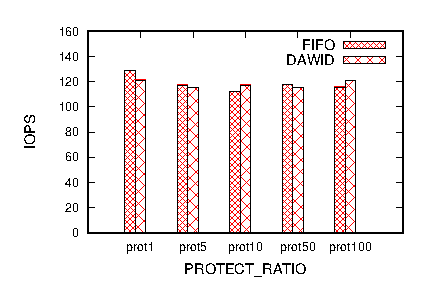
\includegraphics[width=0.3\textwidth]{expr/micro_220517/perf/SEQ/perf_SEQ.eps}
%	} 
%	\subfloat[Random] { 
%	    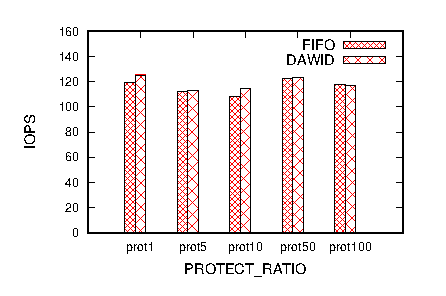
\includegraphics[width=0.3\textwidth]{expr/micro_220517/perf/RAND/perf_RAND.eps}
%	} 
%	\subfloat[JESD] { 
%	    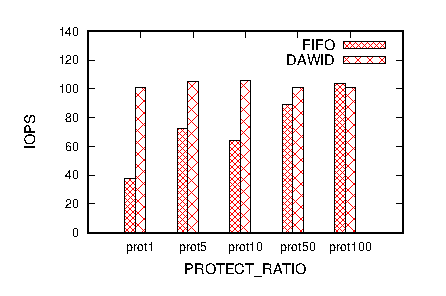
\includegraphics[width=0.3\textwidth]{expr/micro_220517/perf/JESD/perf_JESD.eps}
%	}
%    \caption{\textbf{IOPS}}
%\end{figure*} 
%



